\documentclass[Main.tex]{subfiles} 
\begin{document}

\subsection{Sprint 1}
Sprint 1 fungerede som en typisk elaboration/inception fase fra udviklingsmetoden Unified Process. Her blev sprintet naturligvis brugt til at unders�ge, hvad projektet i bund og grund gik ud p�, s� gruppen fik syn for sagen.
Herefter blev produktopl�gget gransket til hudl�shed, og der blev udformet krav som projektet er bygget p�.
Med et overblik over kravene blev det muligt, at lave en dom�nemodel og akt�rbeskrivelser, samt planl�gge sprintet (vist p� figur \ref{fig:sprint1}).
\\
%\begin{wrapfigure}{r}{0.6\textwidth}
%    \vspace{-20pt}
%  	\centering
%	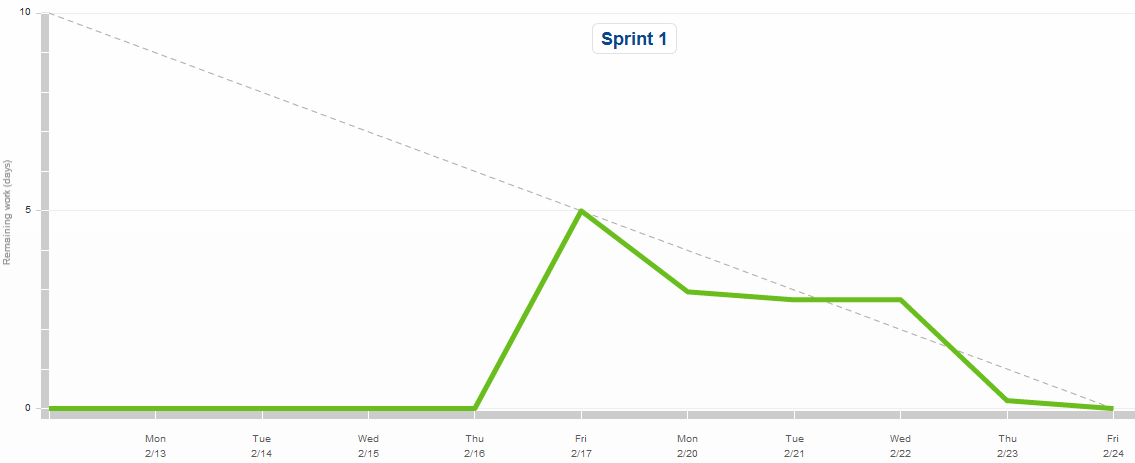
\includegraphics[scale=0.25]{Billeder/Sprint1_burn.png}
%    \vspace{-20pt}
%    \caption{Burndown chart for sprint 1}
%  \label{fig:sprint1}
%  \vspace{-10pt}
%\end{wrapfigure}
Dern�st blev det f�rste udkast til kravspecifikationen p�begyndt. Her benyttede gruppen Use Case-teknikken for at finde akt�rer og deres m�l.
Undervejs blev selve robotten udforsket, s� det var nemmere at danne et overordnet overblik over hvilke funktionaliteter der var n�dvendigt at implementere for at opretholde kravene.
\\
\\
Med et godkendt Use Case-diagram blev en Accepttest p�begyndt og undervejs blev det ligeledes opdaget, at der manglede Use Cases, der tog h�jde for andre scenarier.
\\
\\
I dette sprint blev designet af databasen ogs� p�begyndt. 



\end{document}
